\newpage{\thispagestyle{empty}\cleardoublepage}
\chapter{Introduction} 
\chaptermark{Introduction.} % short title
\label{chap:introduction}
\lettergroup{\thechapter}

\begin{quote}
	\textbf{Abstract:} 
	
	%Recent developments in single-cell transcriptomics have opened new opportunities for studying dynamic processes in immunology in a high-throughput and unbiased manner. Starting from a mixture of cells in different stages of a developmental process, unsupervised trajectory inference algorithms aim to automatically reconstruct the underlying developmental path that cells are following. In this review, we break down the strategies used by this novel class of methods, and organize their components into a common framework, highlighting several practical advantages and disadvantages of the individual methods. We also give an overview of new insights these methods have already provided regarding the wiring and gene regulation of cell differentiation. As the trajectory inference field is still in its infancy, we propose several future developments which will ultimately lead to a global and data-driven way of studying immune cell differentiation.
\end{quote}

\vfill

Partially adapted from:\\
\textbf{Cannoodt, R.}$^*$, Saelens, W.$^*$, and Saeys, Y. Computational methods for trajectory inference from single-cell transcriptomics. \textit{European Journal of Immunology} 46, 11 (2016), 2496--2506. \doi{10.1002/eji.201646347}.\\
Saelens, W.$^*$, \textbf{Cannoodt, R.}$^*$, Todorov, H., and Saeys, Y. A comparison of single-cell trajectory inference methods. \textit{Nature Biotechnology} 37, 5 (2019), 547--554. \doi{10.1038/s41587-019-0071-9}.\\
Todorov, H., \textbf{Cannoodt, R.}, Saelens, W., and Saeys, Y. Network Inference from Single-Cell Transcriptomic Data. \textit{Gene Regulatory Networks} (2019), 235--249. \doi{10.1007/978-1-4939-8882-2_10}. \\
{\footnotesize $^*$ Equal contribution}

\newpage

\section{The cell}
The cell is the smallest unit of life, of which all known living organisms are composed. Every cell houses a plethora of biomolecular processes that allow it to adapt to changes in their environment continuously. It can be very challenging to comprehend the cellular response to a signal due to the dynamic nature of these processes. A reductionist approach to understanding a complex biological system is to study the biochemical components which it is comprised of \cite{brigandt_reductionismbiology_2017}.

Reductionist biologists are delighted by recent advances in experimental technologies that permit measuring the abundance of thousands of different biochemical molecules in tens of thousands of individual cells.  Observing the biomolecular insides of cells in this manner will ultimately provide fundamental insights into the processes that govern these cells and help uncover novel approaches for diagnosing and treating disease. Every coin has its flip side, however, and in this case, it is that the amount of data generated from these experiments is not analysable by hand.  

For example, the Human Cell Atlas (HCA) consortium \cite{regev_humancellatlas_2018} has set out to develop a comprehensive reference map of all the different types of cells in the human body. Experts in the field often metaphorically describe the HCA initiative as aiming to develop a 'Google Maps' of the human body. Even in its infancy, the HCA has profiled 3.8 million cells from 248 donors across 42 labs \cite{humancellatlasconsortium_humancellatlas_2018}, and this number is likely to increase well above one hundred million.

The sheer volume of the data generated from such highly-integrative and high-throughput experiments are not the only reason why they are so challenging to interpret. Namely, the data inherently also suffers from batch effects arising from differences between donors and labs, and also contains high levels of noise arising from the experimental profiling techniques used \cite{hon_humancellatlas_2018}. Biologists thus turn to computer scientists\footnote{or computational biologists turn to themselves} to develop new tools to tackle these problems and help biologists extract meaningful biological insights from the data.

This work makes incremental contributions to the field in order to be able to address the aforementioned problems in a more comprehensive context. This chapter first introduces several key concepts in both cell biology and computer science, upon which the remainder of this work relies. Afterwards, the research objectives and main contributions of this work are outlined.
% TODO: explain that only the main concepts are introduced?

\subsection{The origins of life and the RNA world}
The discovery of the double helix shape of Deoxyribonucleic Acid (DNA) \cite{watson_molecularstructurenucleic_1953} is often considered the pivot point in our understanding of the origins of life and evolution. A modern high-school student can plausibly be expected to know that DNA serves as a medium for storing the genetic information required to reproduce a whole organism. With other words, the DNA of an organism contains the complete set of instructions required to build all of the biomolecular machinery present in its body. The magnitude of this discovery is reflected in our language and culture alike; with sayings such as "It's in your DNA.", or usage of its shape in countless illustrations or artworks (Figure \ref{fig:fsvm}).

\begin{figure}
	\centering
\includegraphics[width=.5\linewidth]{fig/introduction/fsvm3} % TODO: change image
	\caption{
		\textbf{A prominent display of the double helix shape at the VIB FSVM building.} % TODO: expand description
	}
	\label{fig:fsvm}
\end{figure}

Even so, a widely-accepted hypothesis states that life (or cells) did not originate from DNA, but instead was kicked off from its lesser-known cousin, Ribonucleic Acid (RNA). According to the RNA world hypothesis \cite{alberts_rnaworldorigins_2002}, the very first primitive cells used RNA both to store genetic information and perform the chemical reactions required to sustain themselves (Figure \ref{fig:rnaworld}). Only later did cells develop the ability to use DNA and proteins to self-sustain in a process commonly referred to as the Central Dogma.
% TODO: use this reference? \cite{cornell_prebioticaminoacids_2019}

\begin{figure}
	\centering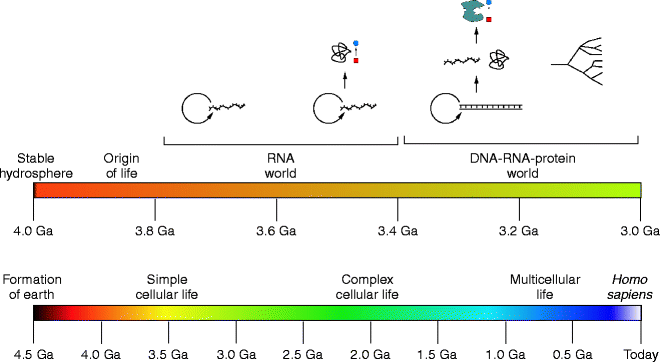
\includegraphics[width=.5\linewidth]{fig/introduction/rnaworld} % TODO: change image
	\caption{
		\textbf{RNA world.} The postulated rise and fall of the RNA world during the evolution of life, from early self-replicating RNA to complex, RNA-controlled metabolism, to the invention of translation, followed by diversification of all modern branches of life. Image from Horning (2011) \cite{horning_rnaworld_2011}. % TODO: expand the description
	}
	\label{fig:rnaworld}
\end{figure}
\subsection{The Central Dogma}
The Central Dogma is a set of processes present which govern the general flow of genetic information in almost all existant living cells. In short, it states that DNA codes for RNA, which in turn codes for proteins. In this work, we assume the main processes involved in the Central Dogma are replication, transcription, splicing and translation (Figure 3). 

\textbf{Replication} is the process of duplicating DNA, which allows a cell to divide such that the resulting daughter cells retain complete copies of its genetic information. DNA consists of four different so-called nucleobases named adenine (A), cytosine (C), guanine (G), and thymine (T). Each strand of the double helix structure of DNA is a linear chain of nucleobases. The two strands are held together by hydrogen bonds since adenine can form three hydrogen bonds with thymine and cytosine can form two hydrogen bonds with guanine. Since each nucleobase can only bond with one other nucleobase, one strand is complementary to the other. Thus a strand of DNA can be represented by a sequence of letters, for example, "ACTCGGTTTAGCA". % This could be part of the DNA explanation.

A stretch of DNA that contains a genetic blueprint for a particular molecule is called a gene, and the collection of an organism's genes is called its genome. \textbf{Transcription} is the process of synthesising an RNA molecule from a gene, and the resulting molecule is called a transcript. RNA is similar to DNA but differs in several ways; most notably all thymine nucleobases are replaced with uracil (U), and RNA molecules consist of only one strand. Due to its single-strandedness, RNA is less stable and will break down faster. Single-strandedness also allows some types of RNA (e.g. transfer RNA, ribosomal RNA) to form more complex three-dimensional structures by having certain regions bind to other regions of the strand. This work only considers messenger RNA (mRNA). mRNAs are transcribed from protein-coding genes, meaning that the mRNAs will lead to the production of protein molecules through the process of translation. 
% TODO: mention that there are about 20'000 protein-coding genes in the human body.

\textbf{RNA splicing} is a process that occurs in almost all organisms (but not all) and results in the removal of specific regions in the RNA molecule. Introns are the regions removed by this process, and exons the regions that remain. The main functionality of splicing is to be able to create multiple variants of the same product, which can affect the enzymatic properties or localisation of the resulting product \cite{kelemen_functionalternativesplicing_2013}.

During \textbf{translation}, a chain of amino acid is synthesised from an mRNA transcript. Every three nucleobases are translated into one of 21 different amino acids. The resulting chain of amino acids is folded up into a protein, the structure of which is determined by the sequence of different amino acids in the chain. In turn, its structure determines the functionality of the protein, which includes catalysing biochemical reactions, providing structure, and transportation of molecules. 
\subsection{Cell types}
The functionality provided by a cell is defined (mostly) by the proteins of which it consists. One common approach to trying to understand the functionality of a cell is to observe which molecules are present in the cell and to associate those molecules with functionality. 

\textit{Homo sapiens} like to categorise everything they encounter and so too have they conceptualised groups of cells called "cell types" according to their functionality. The concept of cell types eases reasoning about all aspects of biology, for instance, which cell types turn into (differentiate) or communicate with which other cell types, or how a cell type responds to a specific stimulation. Cells can be highly specialised toward performing a particular function (e.g. memory B cells accelerate immune response by remembering previously encountered pathogens), while other cells maintain a strong ability to differentiate into other cell types. 

% TODO: do not only discuss differentiation, but instead any kind of developmental process; and mention 'developmental trajectory'.
Cell differentiation is not an instant process; it is a continuous process in which a cell gradually produces the biochemical machinery required in order to fulfil a particular task. In this regard, it makes sense not only to reason about cell types but also about the transition states between cell types and the dynamic processes involved therein.
% TODO: are dynamic processes defined? a dynamic process is just a biochemical reaction

\subsection{Cell dynamics and gene regulation}
If cells are dynamic entities and can gradually produce the molecules needed to acquire new functionality, what is the process by which this happens? The mechanism by which this happens is called gene regulation. Some proteins (or other molecules such as micro RNAs) are capable of determining the rate at which a gene is transcribed (transcription rate). Such proteins are called transcription factors (TFs), and the genes it regulates are called its targets. Typically, one TF will regulate the transcription rate of many targets. % TODO: download database and calculate some statistics.

Production of a specific molecule might require multiple cascades of gene regulation. The collection of all gene regulatory interactions between transcription factors and targets is called a gene regulatory network (GRN). Studying the active parts of a cell's gene regulatory network can thus reveal which dynamic processes are taking place. 

% TODO: explain regulation mechanisms such as transcription factor binding sites?
\subsection{Profiling single cells}
In order to understand a biological process, it is often quite helpful to be able to profile (i.e. observe) the biomolecular components involved therein. The single-cell "omics" technologies which we have at our fingertips today originated from the convergence of two different fields, \emph{"single-cell"} and \emph{"omics"}.

The earliest approaches for measuring the abundance of particular molecules in \emph{single cells} used the preferred instrument of every stereotypical biologist: the microscope. Since it was developed by Coons et al. in 1941, immunohistochemistry (IHC) has been instrumental in visualising antigen-antibody proteins \cite{coons_immunologicalpropertiesantibody_1941}. In many multicellular organisms, antibodies and antigens serve as crucial communication tools as part of the organism's immune system. A cell can present a particular type of antigen on its cell surface, which allows a particular type of antibody to bind to it.

IHC (and many other biotechnologies) visualises antigen-antibody reactions by attaching particular molecules to the antibody, such as an enzyme that catalyses a colour-producing reaction, or a fluorescent chemical compound that can re-emit light upon light excitation. Using different colours (wavelengths) allows measuring expression levels of different antibodies simultaneously. Characterising cells in a quantifiable way is labour intensive; however, since it involves acquiring an image of many cells and drawing a contour around each cell (called cell segmentation). While modern implementations of IHC improve the throughput drastically by using robots to automate the image acquisition and computer software to automate cell segmentation, the procedure is still labour intensive as the robots and computer software still needs to be kept in check.

Flow cytometry \cite{fulwyler_electronicseparationbiological_1965} is a technique which circumvents imaging and segmentation issues by having a steady stream of cells run through a laser and measuring the amount of light scattered from those cells. Flow cytometry technology enables to measure protein expression levels for millions of cells and tens of different antibodies. 

Since IHC and flow cytometry, many new technologies have been developed which allow quantifying expression levels of molecules in single cells (e.g. mass cytometry, single-cell qPCR, FISH). All of these single-cell (non-omics) technologies are limited by the number of different molecules they could measure, however; and thus required handpicking the molecules of interest before performing an experiment, making the experiment biased towards the preconceptions of the experimenter.

On the other side of the spectrum are the so-called "omics" technologies. "Omics"\footnote{The etymology of "omics" is quite interesting \cite{yadav_wholenesssuffixomics_2007}.} is a collective term for profiling all molecules of a particular type in a high-throughput manner. There are many types of "omics", but the most commonly used are the following. In genomics, all of an organism's genes are studied -- its whole genome. Transcriptomics and proteomics study the organisms RNA transcripts and proteins, respectively. A notable downside of traditional omics technologies is that in order to capture enough material an ensemble of cells needs to be profiled, and thus only the average expression levels are returned; thereby granting the technology the name "bulk" omics. If a subset of these cells contains unique patterns in expression levels, this pattern will be masked in the bulk population and is thus undetectable. Specific examples of omics technologies are next-generation sequencing, which can be used to determine the DNA sequence of an organism, and RNA sequencing, which profiles the sequences of RNA transcripts. By mapping the sequences of RNA transcripts to genes in the organisms DNA, a gene expression profile can be obtained.
% Demonstrate the masking effect of bulk analyses.

Transformative technological advances in microvolume sequencing allowed Tang et al. to analyse the transcriptome at single-cell resolution \cite{tang_mrnaseqwholetranscriptomeanalysis_2009}, thereby bringing single-cell biology and omics together to create single-cell omics (Figure \ref{fig:profiling_convergence}A). During the decade that followed, the number of single-cell omics technologies has skyrocketed, allowing to profile tens of thousands of cells (Figure \ref{fig:profiling_convergence}B) and measuring other levels of information such as proteomic expression levels (Figure \ref{fig:profiling_convergence}C).

\begin{figure}
	\centering
	A. 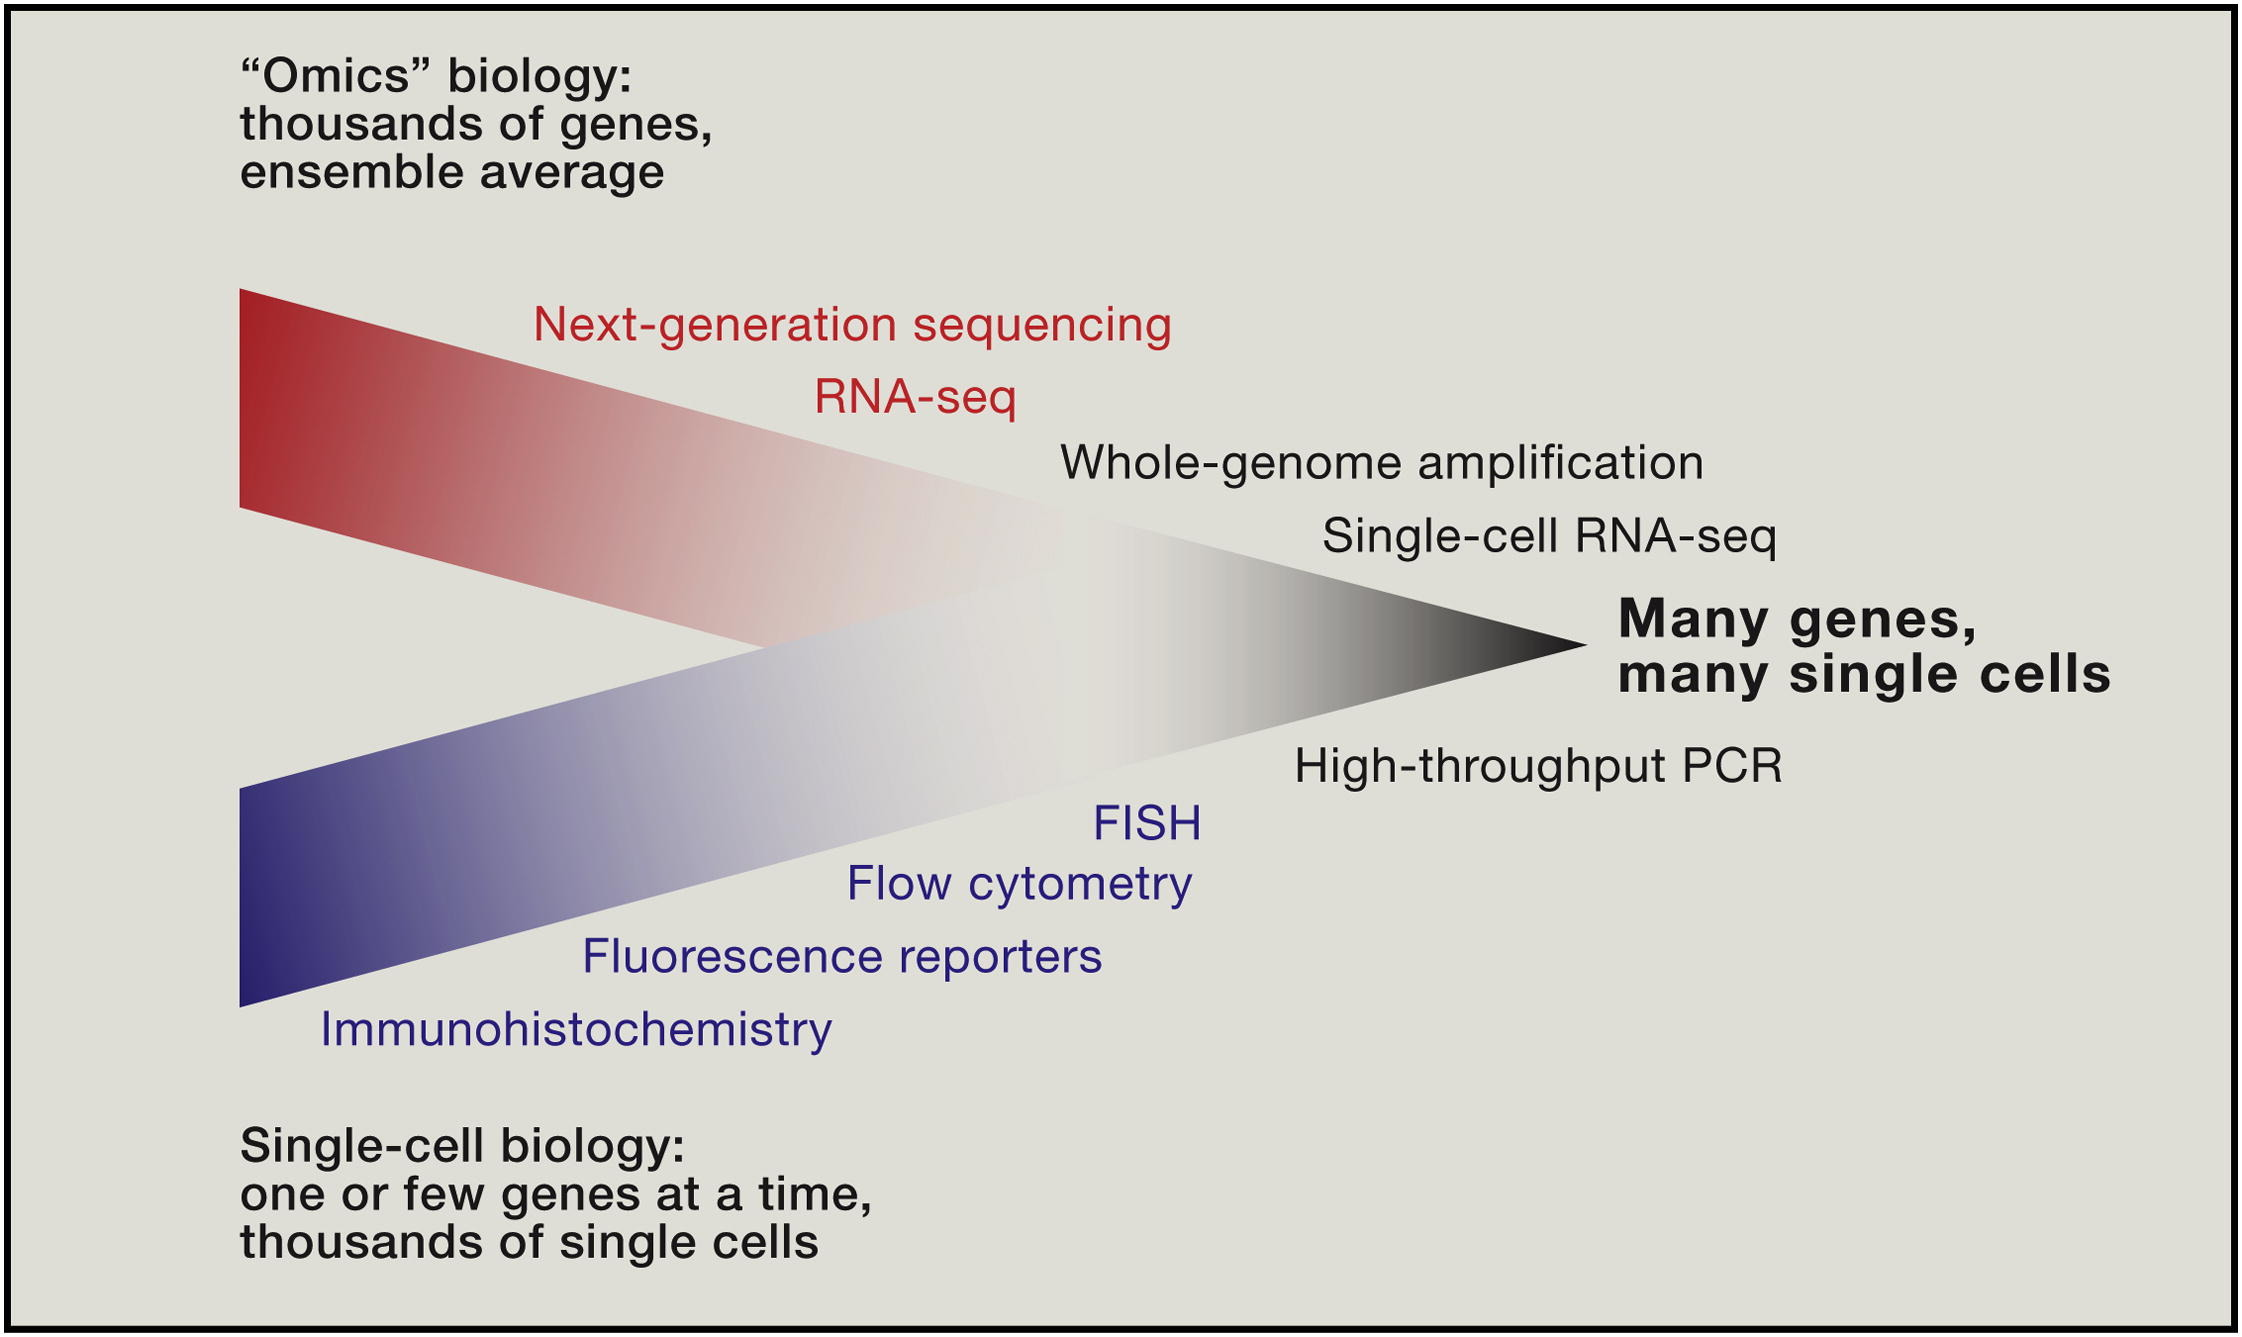
\includegraphics[width=.45\linewidth]{fig/introduction/profiling_convergence} 
	% also figure with cell numbers
	C. 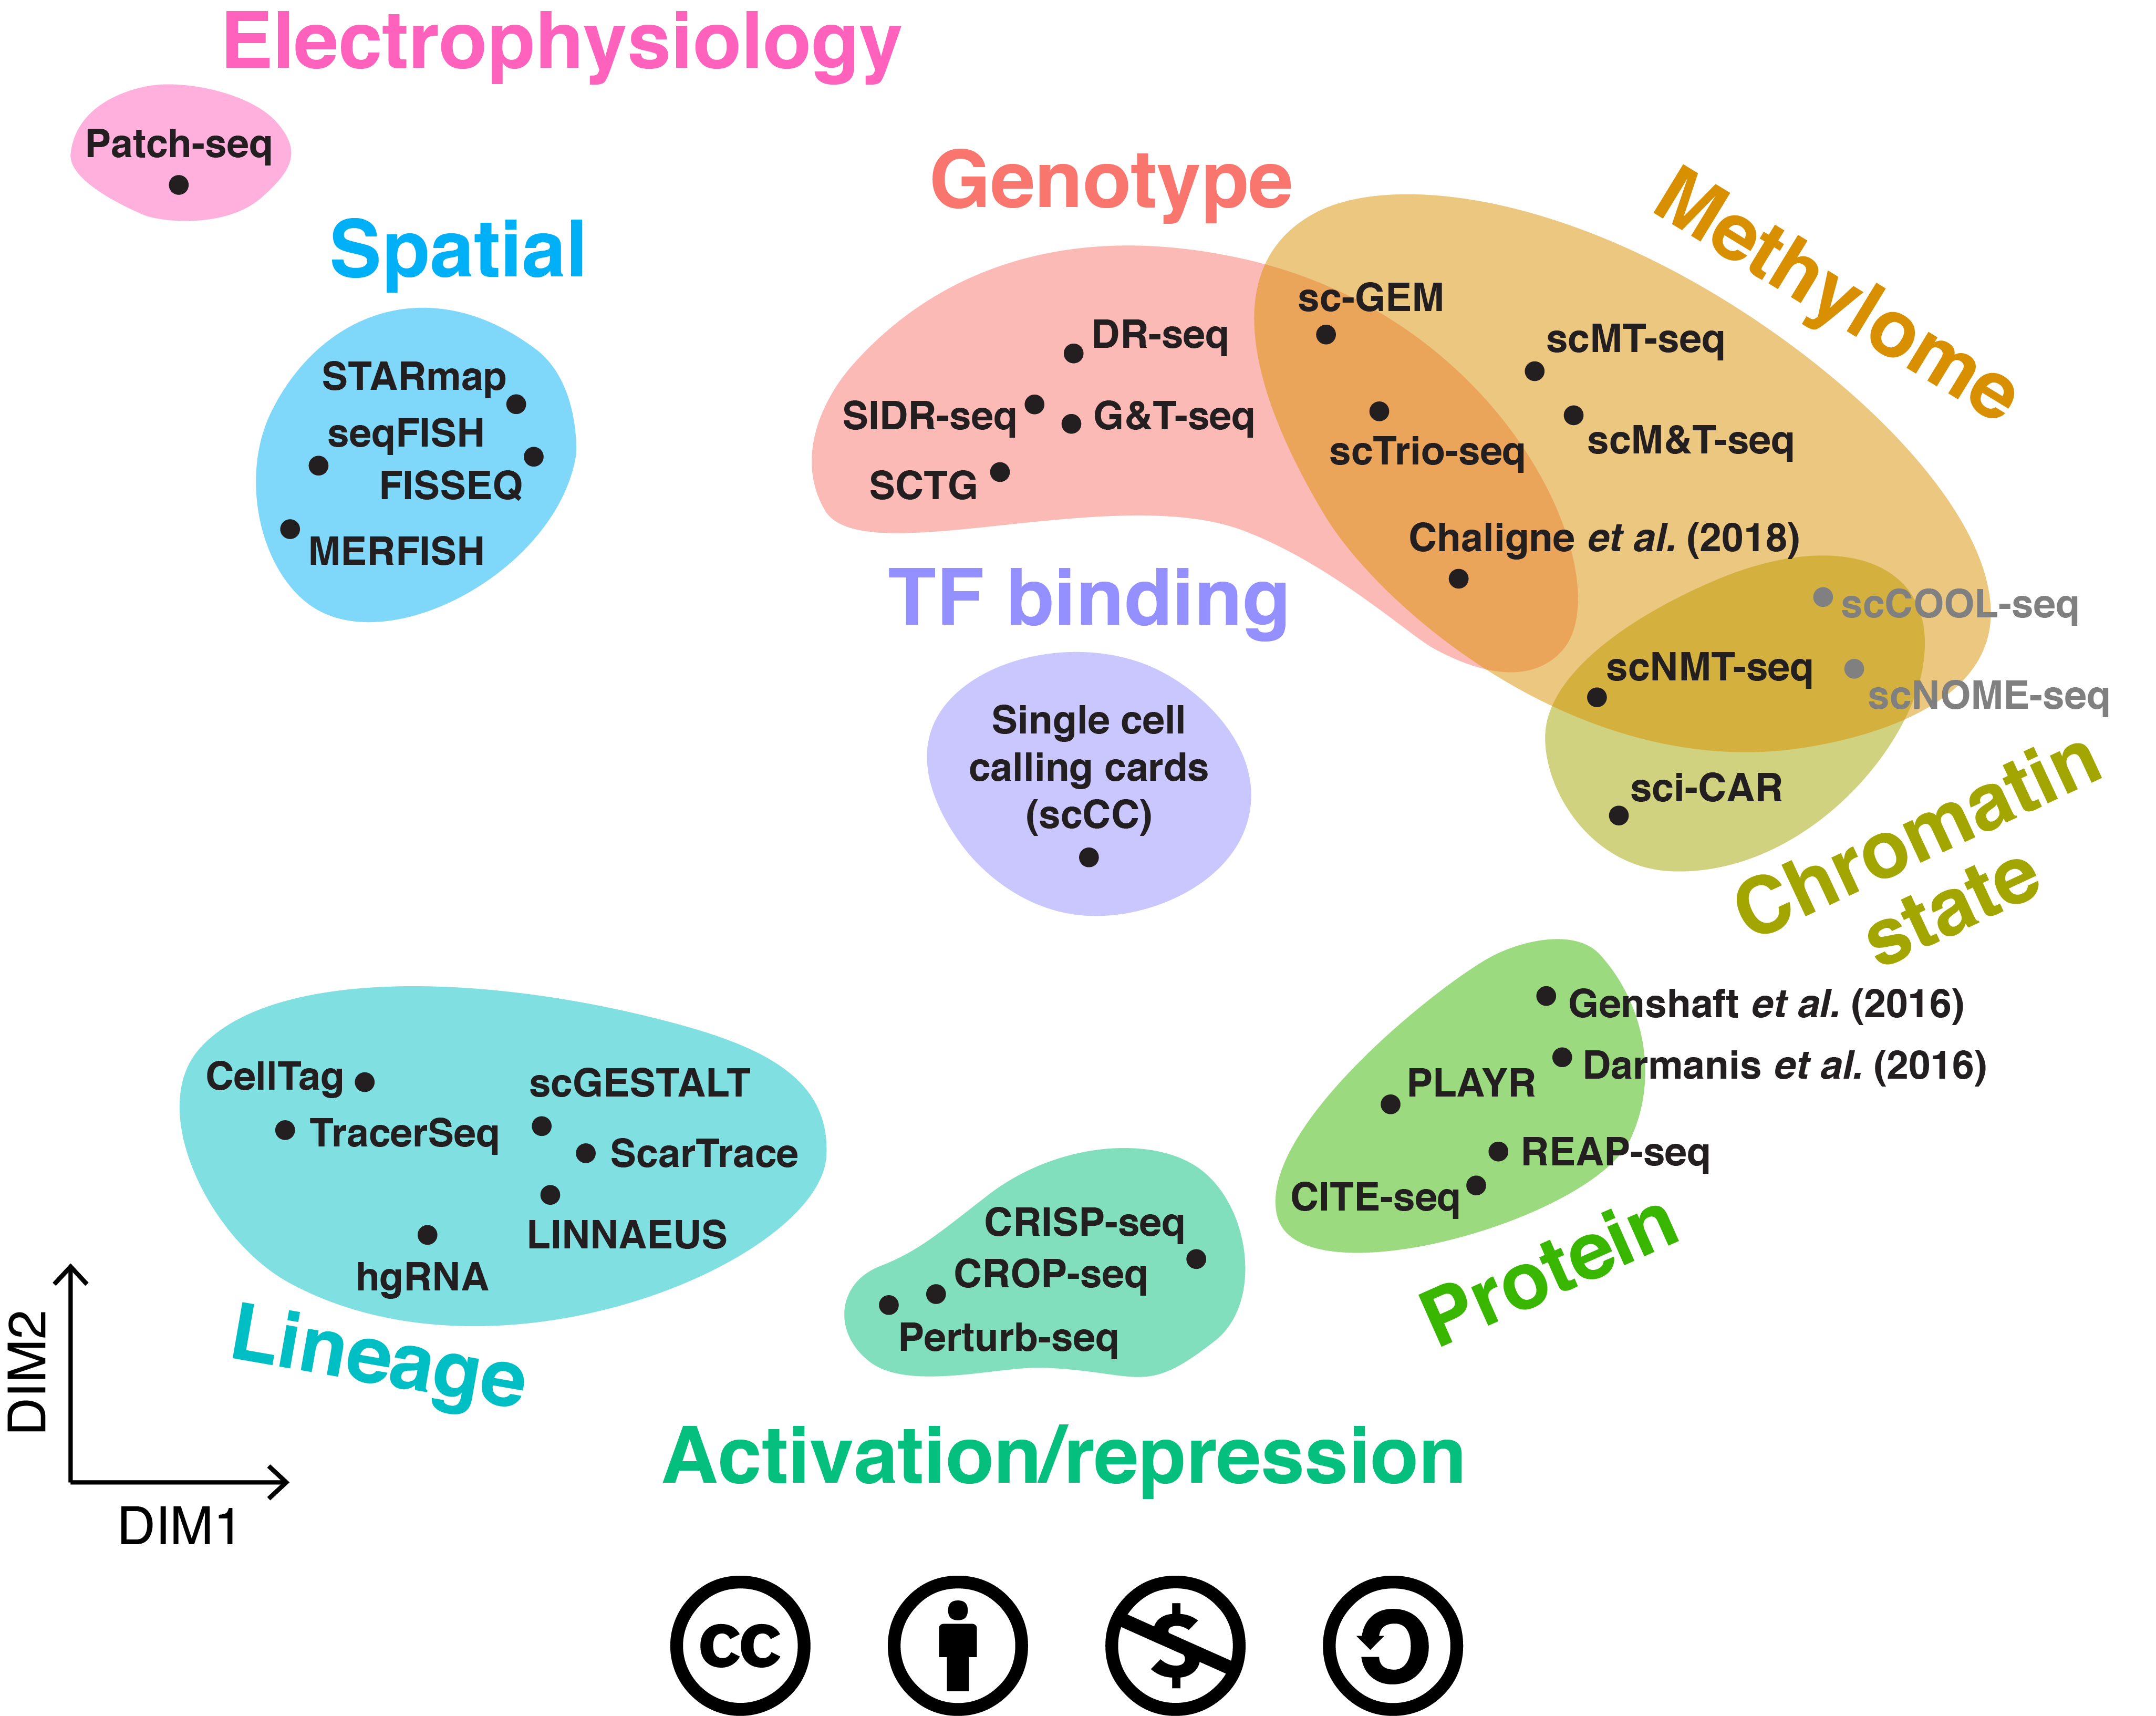
\includegraphics[width=.45\linewidth]{fig/introduction/multimodal} 
	% TODO: change image
	\caption{
		A. \textbf{Convergence of "Omics" Biology and Single-Cell Biology.} Technology that allows researchers to obtain genome-wide information from single cells is extending the boundaries of a field that has thus far been limited to the analyses of a select gene in eukaryotes. Image from Junker and van Oudenaarden (2014) \cite{junker_everycellspecial_2014}. 
		B. 
		C. scmultiomics \cite{moudgil_multimodalscrnaseq_2019}. 
		% TODO: rewrite the description
	}
	\label{fig:profiling_convergence}
\end{figure}

The rapidly advancing field of single-cell omics harbours exceptional opportunities to discover new aspects of biology and redefine existing knowledge. Some of these opportunities lie in efforts like the Human Cell Atlas. The HCA consortium has set out to redefine all human cell types in terms of their gene expression and location, and the developmental trajectories connecting the different cell types. As part of this endeavour, the consortium will likely profile the whole transcriptomes tens or even hundreds of millions of cells. 

\section{Computational tools}
The rapidly advancing field of single-cell omics harbours exceptional opportunities to discover new aspects of biology and redefine existing knowledge. 

Some of these opportunities lie in efforts such as the Human Cell Atlas. The HCA consortium has set out to redefine all human cell types in terms of their gene expression and location, and the developmental trajectories which connect the different cell types. As part of this endeavour, the consortium will perform single-cell omics on tens or even hundreds of millions of cells.

Single-cell omics permits new types of analyse but also come with hitherto unseen data characteristics, the combination of which poses exciting new challenges for the computational community to tackle (Figure \ref{fig:comp_tools}A)\cite{stegle_computationalanalyticalchallenges_2015,yuan_challengesemergingdirections_2017,chen_singlecellrnaseqtechnologies_2019}. These challenges include:
\begin{itemize}
	\item normalisation: separating biological noise from technical noise,
	\item dimensionality reduction: providing a visual and informative overview of a given dataset, 
	\item trajectory inference: identifying and characterising transitions between different cellular states, and
	\item gene regulatory network inference: inferring regulatory interactions between transcription factors across individual cells.
\end{itemize}

\begin{figure}
	\centering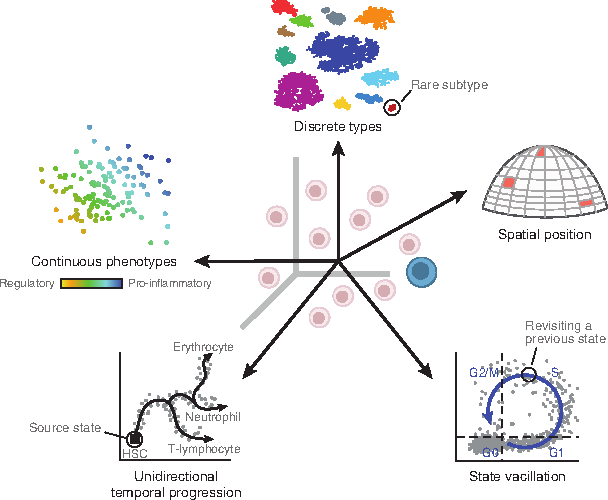
\includegraphics[width=.5\linewidth]{fig/introduction/singlecell_tools}
	\centering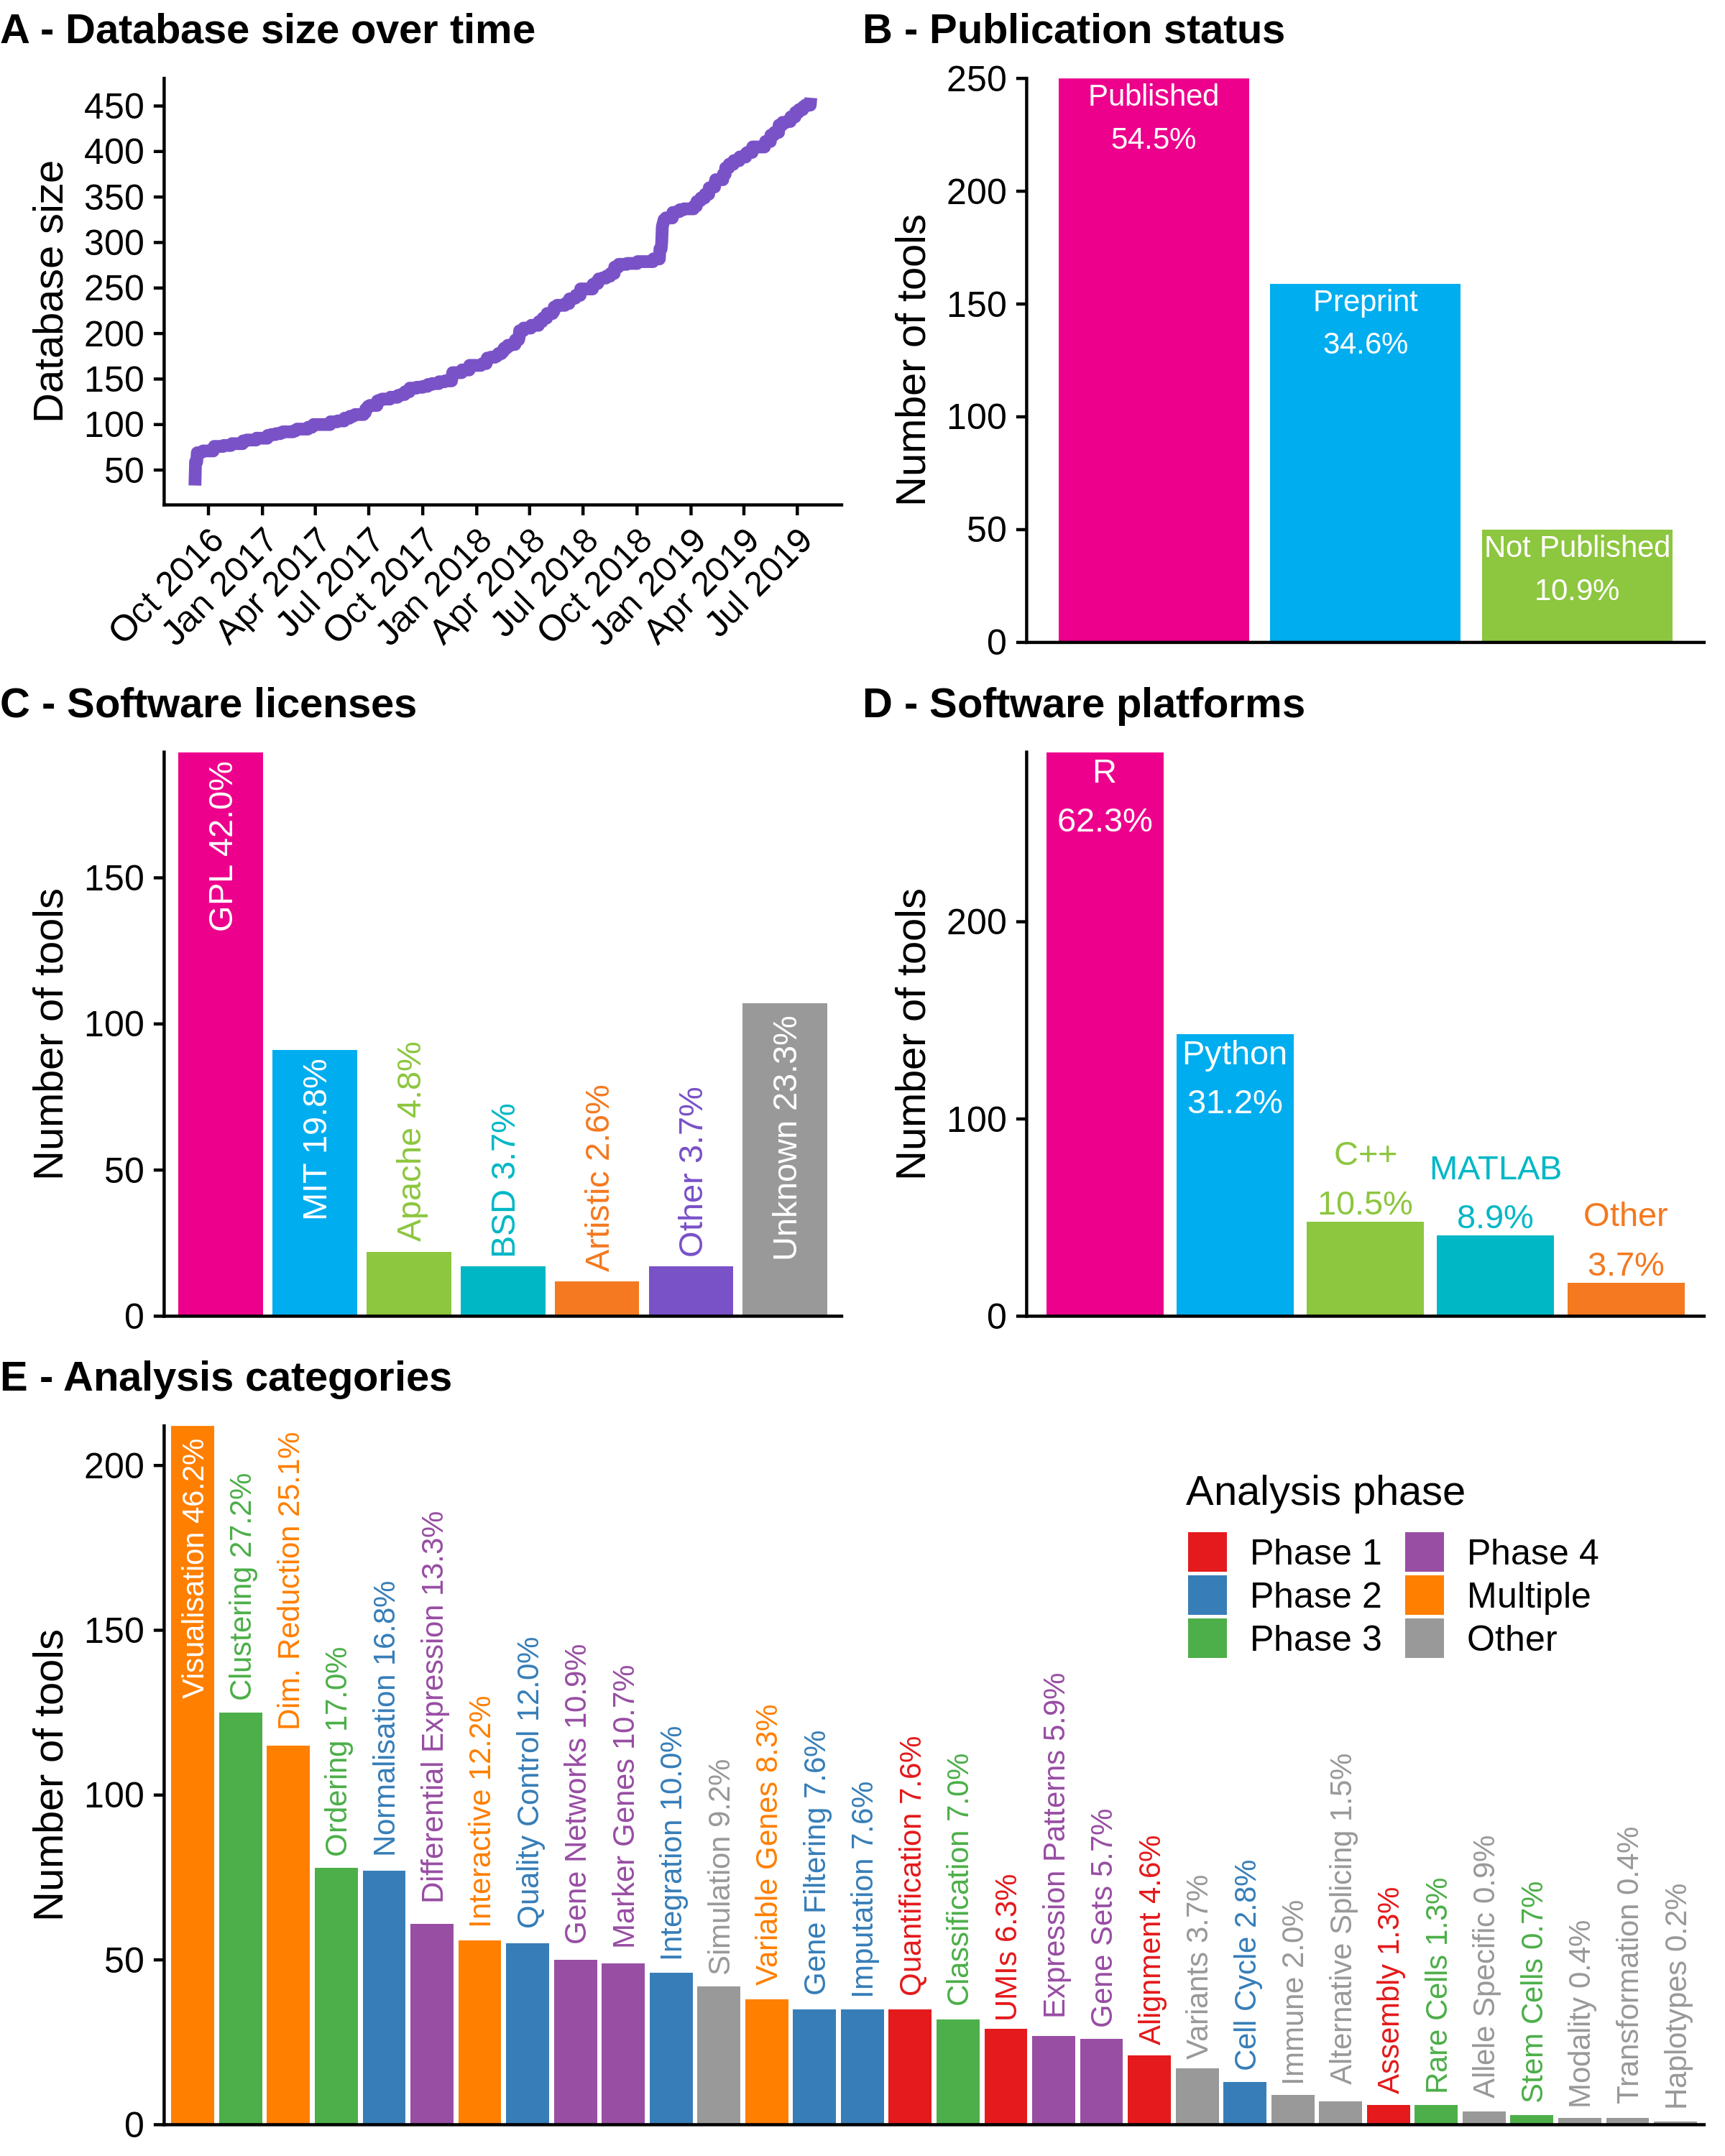
\includegraphics[width=.3\linewidth]{fig/introduction/scrnatools}
	% TODO: change image
	\caption{\textbf{A. Single-cell omics allows for many new types of computational approaches.} Figure adapted from Wagner et al. (2016) \cite{wagner_revealingvectorscellular_2016}.
		B. Zappia et al. (2018) \cite{zappia_exploringsinglecellrnaseq_2018}
		% TODO: rewrite the description
	}
	\label{fig:comp_tools}
\end{figure}

% TODO: provide better connection to the subsections below

\subsection{Normalisation}
% TODO: need to write still

\subsection{Dimensionality reduction}
Single-cell omics datasets typically have too many dimensions (features) in order to be easily interpretable by humans and even by most computational tools. 
Dimensionality reduction (DR) methods transform high-dimensional data into a meaningful representation with fewer dimensions. It is important to note that its usage depends on the target audience: for humans -- to visualise data in a 2-D plane to aid with interpretation by humans, or for computers -- to construct a denser representation of the data such that it mostly contains the same information but with fewer dimensions.

There are many ways of classifying DR methods \cite{engel_surveydimensionreduction_2012}, but this work will use the following main categories: feature projection-based and manifold learning. 
Projection-based DR methods aim to perform a linear transformation of the data while preserving the pairwise distances between samples as much as possible. Examples of commonly used projection-based DR methods in single-cell omics are PCA and MDS. 
Manifold learning methods are methods which reconstruct a higher-order structure in the original space (e.g. a graph or a grid), visualising the structure in a lower-dimensional space, and mapping the original samples to the lower-dimensional space. Manifold learning can be an iterative optimisation process using a predefined criterion. Examples of manifold learning techniques are t-SNE, Diffusion Maps and UMAP. 
% section is not very interestingly written

\subsection{Trajectory inference}
Single-cell omics data provide new opportunities for studying cellular dynamic processes, such as the cell cycle, cell differentiation and cell activation \cite{tanay_scalingsinglecellgenomics_2017,etzrodt_quantitativesinglecellapproaches_2014}. 
Trajectory inference (TI) is a new category of computational tools used to offer an unbiased and transcriptome-wide understanding of a dynamic process \cite{tanay_scalingsinglecellgenomics_2017,cannoodt_computationalmethodstrajectory_2016}. 

The dataset can be a single snapshot of a mixture of cells in different stages, or a set of samples collected at different time points (Figure \ref{fig:trajectory_inference}A). Typically, TI methods first analyse similarities between cells, optionally infer the topology of the underlying process, and finally order cells along that trajectory (Figure \ref{fig:trajectory_inference}B). The second step can be optional, as some methods assume a specific topology beforehand.
TI methods allow the identification of new subsets of cells, delineation of a differentiation tree, and characterisation of the main driver genes along a state transition (Figure \ref{fig:trajectory_inference}C). Current applications of TI focus on specific subsets of cells, but ongoing efforts to construct transcriptomic catalogs of whole organisms \cite{regev_humancellatlas_2017,han_mappingmousecell_2018,schaum_singlecelltranscriptomics20_2018} underline the urgency for accurate, scalable \cite{aibar_scenicsinglecellregulatory_2017,angerer_singlecellsmake_2017} and user-friendly TI methods.

\begin{figure}
	\centering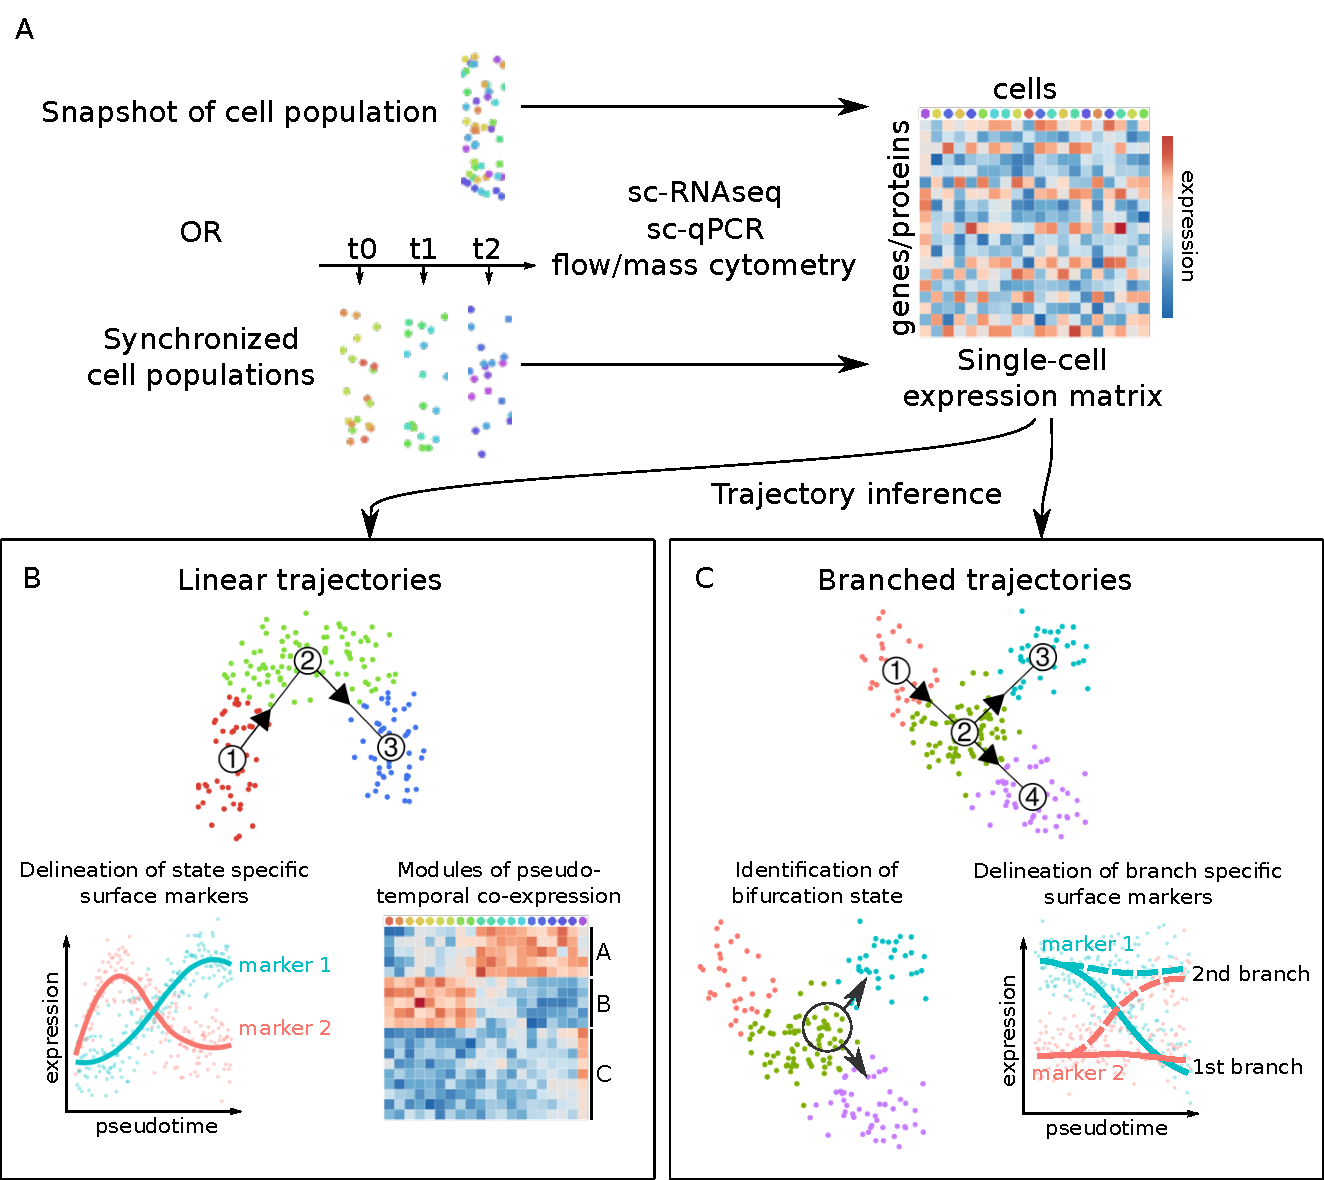
\includegraphics[width=\Largefigure]{fig/introduction/trajectory_inference_slim} % TODO: Update figure to match text!!!!
	\caption{
		Applications of single-cell trajectory inference methods. (A) Single-cell omics data appropriate for TI can be both obtained from an unsynchronised population of single cells (snapshot data) but also from synchronised cell populations. (B) UPDATE! (C) UPDATE!
	}
	\label{fig:trajectory_inference}
\end{figure}


\subsection{Gene regulatory network inference}
Gene regulatory network inference, or network inference (NI) for short, is a type of computational analysis where thousands of transcriptomic profiles are analysed together in order to infer the regulatory interactions between transcription factors and genes. This topic already received much attention with the advent of bulk omics (before single-cell omics). These efforts culminated in several DREAM competitions assessing the performance of 29 different NI methods \cite{marbach_revealingstrengthsweaknesses_2010, marbach_wisdomcrowdsrobust_2012}. 

After the last DREAM competition, it seemed that interest in NI methodology had declined. After all, NI on bulk omics profiles suffered from several crucial issues. As mentioned previously, bulk profiles are generated by pooling together the RNA transcripts of a supposedly homogeneous population of thousands of cells. Since the expression values are averaged over the whole population, incorrect assumptions on the homogeneity of the pooled cells may lead to the masking of relevant expression patterns in rare cell populations (Figure \ref{fig:bulk_vs_singlecell}). Besides, NI methods rely on a diverse set of time-series and perturbation experiments in order to reliably identify causal regulatory interactions. Such experiments are expensive and time-consuming, and an inaccurate selection of time points might result in crucial intermediate stages being missed.

\begin{figure}
	\centering
	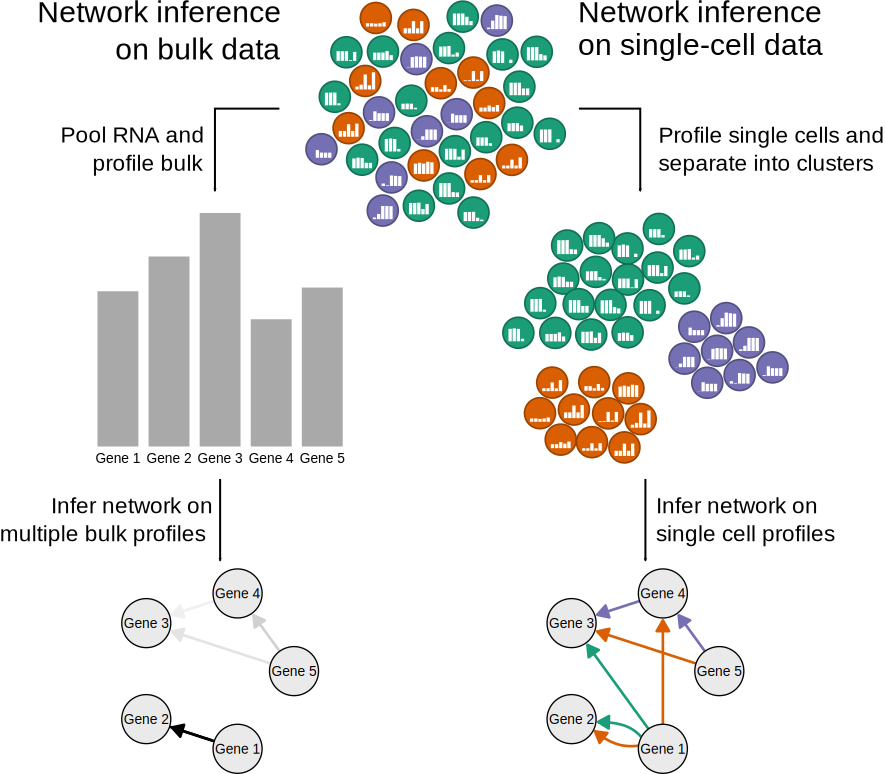
\includegraphics[width=\Largefigure]{fig/introduction/ni_bulk_vs_sc}
	\caption{Bulk expression data return the average expressions of genes among large numbers of cells. In order to infer regulatory networks from this type of data, multiple bulk profiles (resulting from time series or perturbation experiments) are required. On the other hand, sequencing the transcriptome at the single-cell level uncovers the high variability among cells, providing the necessary information to infer gene regulatory networks directly.} % TODO: update label
	\label{fig:bulk_vs_singlecell}
\end{figure}

The advent of single-cell omics has made scientists wonder whether now is the time to revisit network inference \cite{stegle_computationalanalyticalchallenges_2015}. 
One of the main advantages of single-cell omics is the ability to quantify the exact cellular state of thousands of cells per experiment. The heterogeneity between cells caused by naturally occurring biological randomness \cite{padovan-merhar_usingvariabilitygene_2013} can be exploited to infer regulatory interactions between TFs and their target genes at much lower costs (see Figure \ref{fig:bulk_vs_singlecell}).
In this setting, heterogeneity in the cell population eases network inference, rather than mask condition-specific expression patterns in regulatory interactions.

\section{Research objectives}

Recent technological advancements in profiling single cells are having significant repercussions in many fields of biology. The new types of analyses made possible warrant the development of computational tools which can solve the problem at hand and deal with the new data characteristics, ultimately in order to create useful and accurate hypotheses for biologists.

In response, scientists all over the globe have been working hard to tackle these computational challenges, resulting in more than 470 software tools for processing single-cell omics data in one form or another \cite{zappia_exploringsinglecellrnaseq_2018}. More than half of these tools were published in peer-reviewed journals. 

The high number of tools available presents the user choice, but also uncertainty and indecision about which tool to use for the task at hand. Choosing the method with most citations might result in a weaker result than picking a method at random, and making an informed decision requires spending an enormous amount of time in comparing the results of numerous methods, on various platforms, on multiple different datasets. 

The field of single-cell omics needs quantitative ways to measure the performance of different categories of tools. Clear quantitative metrics allow performing comprehensive studies to assess the advantages and disadvantages of existing tools. In addition, they could also serve as a minimum performance criterion before the publication of a new tool.

In the computational jungle of single-cell omics, experts act as beacons of hope by sharing guidelines based on comprehensive benchmarking studies. Their disseminations (in the form of manuscripts \cite{lafzi_tutorialguidelinesexperimental_2018,luecken_currentbestpractices_2019}, courses \cite{kiselev_analysissinglecell_2019,martens_analysissinglecell_2019}, and slides shown during keynote caffeine refuelling sessions \cite{hemberg_coffeebreakanalysis_2019}) are crucial in leading new users, and ultimately the whole field, to better practices for performing single-cell omics analyses.

% todo: provide better segway to the next section

\section{Outline} % include contributions?
This work aims to tackle multiple computational problems in extracting biological hypotheses from single-cell omics data.
We introduce a framework for evaluating multiple types of single-cell omics tools, more specifically dimensionality reduction, trajectory inference, and gene regulatory network inference (Chapter \ref{chap:dyngen}). Next, we perform a comprehensive evaluation of 45 TI methods and construct guidelines based on our observations (Chapter \ref{chap:dynbenchmark}). As part of the evaluation, we developed a framework to infer, visualise, and interpret trajectories, which we made available as a separate tool called dyno (Chapter \ref{chap:dyno}).
We also introduce two new computational tools of our own. SCORPIUS is a TI method specialised in inferring linear trajectories (Chapter \ref{chap:scorpius}). bred is a true single-cell NI method which can infer gene regulatory networks for individual cells (Chapter \ref{chap:bred}).

\textbf{Chapter \ref{chap:dyngen}} -- why dyngen, what is it, what can it be used for.
%framework for evaluating methods with synthetic data generator. if available, real data with gold standards would be most desirable.

\textbf{Chapter \ref{chap:dynbenchmark}} -- why dynbenchmark, what is it, what can it be used for.

\textbf{Chapter \ref{chap:dyno}} -- why dyno, what is it, what can it be used for.

\textbf{Chapter \ref{chap:scorpius}} -- why scorpius, what is it, what can it be used for.

\textbf{Chapter \ref{chap:bred}} -- why bred, what is it, what can it be used for.



%Before embarking on this perilous adventure, I attempt to write a "Hippocratic oath for bioinformaticians", to guide me through this dissertation and not stray from the metaphorical path of righteousness.
%
%\subsection{Hippocratic oath for bioinformaticians}
%We proceed with caution in developing new tools. Its results should not only be convincing and easy to interpret, but also accurate, robust, and reproducible. We value creating open-source software that works reliably but fails gracefully when it does not. We acknowledge that writing automated tests is dull but necessary for maintaining long-term software projects. % TODO: improve

\section{List of contributions}

\subsection{First-author publications}

\begin{itemize}
	\item \textbf{Cannoodt R} *, Saelens W *, Saeys Y. Computational methods for trajectory inference from single-cell transcriptomics. European journal of immunology. 2016 Nov;46(11):2496-506.
	\item \textbf{Cannoodt R}, Saelens W, Sichien D, Tavernier S, Janssens S, Guilliams M, Lambrecht B, De Preter K, Saeys Y. SCORPIUS improves trajectory inference and identifies novel modules in dendritic cell development. bioRxiv. 2016 Oct:079509.
	\item \textbf{Cannoodt R}, Ruyssinck J, Ramon J, De Preter K, Saeys Y. IncGraph: Incremental graphlet counting for topology optimisation. PloS one. 2018 Apr 26;13(4):e0195997.
  \item Saelens W *, \textbf{Cannoodt R} *, Todorov H, Saeys Y. A comparison of single-cell trajectory inference methods. Nature biotechnology. 2019 May;37(5):547.
  \item dyngen, submitted?
  \item dyno, submitted?
  \item scorpius, submitted?
  \item bred, submitted?
 \end{itemize}

*: Equal contribution.

\subsection{Co-author publications}
\begin{itemize}
	\item Decock A, Ongenaert M, \textbf{Cannoodt R}, Verniers K, De Wilde B, Laureys G, Van Roy N, Berbegall AP, Bienertova-Vasku J, Bown N, Clément N. Methyl-CpG-binding domain sequencing reveals a prognostic methylation signature in neuroblastoma. Oncotarget. 2016 Jan 12;7(2):1960.
	\item Van Cauwenbergh C, Van Schil K, \textbf{Cannoodt R}, Bauwens M, Van Laethem T, De Jaegere S, Steyaert W, Sante T, Menten B, Leroy BP, Coppieters F. arrEYE: a customized platform for high-resolution copy number analysis of coding and noncoding regions of known and candidate retinal dystrophy genes and retinal noncoding RNAs. Genetics in Medicine. 2017 Apr;19(4):457.
	\item Claeys S, Denecker G, \textbf{Cannoodt R}, Kumps C, Durinck K, Speleman F, De Preter K. Early and late effects of pharmacological ALK inhibition on the neuroblastoma transcriptome. Oncotarget. 2017 Dec 5;8(63):106820.
	\item Depuydt P, Boeva V, Hocking TD, \textbf{Cannoodt R}, Ambros IM, Ambros PF, Asgharzadeh S, Attiyeh EF, Combaret V, Defferrari R, Fischer M. Genomic amplifications and distal 6q loss: novel markers for poor survival in high-risk neuroblastoma patients. JNCI: Journal of the National Cancer Institute. 2018 Mar 5;110(10):1084-93.
	\item Scott CL, T'Jonck W, \ldots, \textbf{Cannoodt R}, Saelens W \ldots, Guilliams M. The transcription factor ZEB2 is required to maintain the tissue-specific identities of macrophages. Immunity. 2018 Aug 21;49(2):312-25.
	\item Saelens W, \textbf{Cannoodt R}, Saeys Y. A comprehensive evaluation of module detection methods for gene expression data. Nature communications. 2018 Mar 15;9(1):1090.
	\item Todorov H, \textbf{Cannoodt R}, Saelens W, Saeys Y. Network Inference from Single-Cell Transcriptomic Data. InGene Regulatory Networks 2019 (pp. 235-249). Humana Press, New York, NY..
	\item Van den Berge K, De Bezieux HR, Street K, Saelens W, \textbf{Cannoodt R}, Saeys Y, Dudoit S, Clement L. Trajectory-based differential expression analysis for single-cell sequencing data. BioRxiv. 2019 Jan 1:623397.
	\item Weber LM, Saelens W, \textbf{Cannoodt R}, Soneson C, Hapfelmeier A, Gardner PP, Boulesteix AL, Saeys Y, Robinson MD. Essential guidelines for computational method benchmarking. Genome biology. 2019 Dec;20(1):125.
\end{itemize}

\subsection{Open-source software}
As part of this work, many open-source software packages were created and many others were contributed to (Table \ref{tab:packages}). 

Packages that were created as part of this work are hosted on Github under the username rcannood\footnote{\url{https://github.com/rcannood?tab=repositories}} or the dynverse organisation\footnote{\url{https://github.com/dynverse?tab=repositories}}. As part of our standard development practices, we automate execution of unit tests and writing extensive documentation to ensure the code complies with CRAN policy before submission. We aim to submit all other packages to CRAN as well.

We also helped maintain or extend other packages on Github, CRAN or Bioconductor on which our software depends. This includes help speed up parts of the dependency (slingshot), adding new functionality (devtools, ParamHelpers), fixing bugs (proxyC, rlang, monocle, splatter, slingshot), becoming a maintainer of orphaned packages (princurve, GillespieSSA), and extending the documentation (devtools, mlr, remotes). Several of these package receive millions of downloads per year (devtools, remotes, rlang).

\newcommand{\cranpkg}[1]{\href{https://cran.r-project.org/package=#1}{#1}}
\newcommand{\biocpkg}[1]{\href{https://bioconductor.org/packages/#1}{#1}}
\newcommand{\biocpkgl}[2]{\href{https://bioconductor.org/packages/#1}{#2}}
\newcommand{\githubpkg}[2]{\href{https://github.com/#1/#2}{#2}}
\newcommand{\notavailable}{}

%library(dlstats)
%library(tidyverse)
%
%cran <- c("babelwhale", "dyndimred", "dynparam", "dynutils", "GillespieSSA", "GillespieSSA2", "incgraph", "princurve", "proxyC", "qsub", "SCORPIUS", "devtools", "mlr", "ParamHelpers", "remotes", "rlang")
%bioc <- c("ClusterSignificance", "monocle", "slingshot", "splatter")
%
%dl_cran <- dlstats::cran_stats(cran)
%dl_bioc <- dlstats::bioc_stats(bioc)
%
%dls <- bind_rows(dl_cran, dl_bioc %>% select(start, end, package, downloads = Nb_of_downloads)) %>% 
%mutate(role = ifelse(package %in% c("devtools", "mlr", "ParamHelpers", "remotes", "rlang", bioc), "Contributor", "Author"))
%
%summ <- dls %>% filter("2019-08-01" <= start) %>% group_by(package) %>% summarise(downloads = sum(downloads) / 23 * 365)
%
%summ <- dls %>% filter("2018-07-01" <= start, end <= "2019-07-30") %>% group_by(package) %>% summarise(downloads = sum(downloads))


\begin{table}[ht!]
	\caption{\textbf{Contibutions to open-source software.} Following abbreviations denote the role within the package: aut Author, ctb Contributor. Yearly download statistics are based on the number of downloads between 2019-08-01 and 2019-08-23. CRAN download statistics are retrieved from the Rstudio CRAN mirror only; other CRAN mirrors do not track download statistics. For Github repositories, no download statistics could be retrieved. } \label{tab:packages}
	
	\centering\fontsize{9}{11}\selectfont
	\begin{tabularx}{\linewidth}{|p{2cm}llp{1.5cm}X|}
		\hline
		Name & Role & Host & Downloads per year & Description \\ \hline\hline
		\cranpkg{babelwhale} & aut & CRAN & 3491 & Interacting with Docker and Singularity containers \\
		\githubpkg{dynverse}{dynbenchmark} & aut & Github & \notavailable & Pipeline for benchmarking trajectory inference methods \\
		\cranpkg{dyndimred} & aut & CRAN & 571 & Applying dimensionality reduction methods \\
		\githubpkg{dynverse}{dyneval} & aut & Github & \notavailable & Evaluating trajectory inference methods \\
		\githubpkg{dynverse}{dynfeature} & aut & Github & \notavailable & Calculating feature importance scores from trajectories \\
		\githubpkg{dynverse}{dyngen} & aut & Github & \notavailable & Simulating single-cell data using gene regulatory networks \\
		\githubpkg{dynverse}{dynguidelines} & aut & Github & \notavailable & User guidelines for trajectory inference \\
		\githubpkg{dynverse}{dynmethods} & aut & Github & \notavailable & A collection of wrappers for trajectory inference methods \\
		\githubpkg{dynverse}{dyno} & aut & Github & \notavailable & A pipeline for inferring, visualising and interpreting trajectories \\
		\cranpkg{dynparam} & aut & CRAN & 2539 & Creating meta-information for parameters \\
		\githubpkg{dynverse}{dynplot} & aut & Github & \notavailable & A simple visualisation library for trajectories \\
		\githubpkg{dynverse}{dynplot2} & aut & Github & \notavailable & A fully customisable visualisation library for trajectories \\
		\githubpkg{dynverse}{dyntoy} & aut & Github & \notavailable & Generating simple toy data of cellular differentiation \\
		\cranpkg{dynutils} & aut & CRAN & 4570 & Common functionality for the dynverse packages \\
		\githubpkg{dynverse}{dynwrap} & aut & Github & \notavailable & A common format for trajectories \\
		\cranpkg{GillespieSSA} & aut & CRAN & 7855 & Gillespie's Stochastic Simulation Algorithm (SSA) \\
		\cranpkg{GillespieSSA2} & aut & CRAN & 2253 & Gillespie's Stochastic Simulation Algorithm for Impatient People \\
		\githubpkg{dynverse}{gng} & aut & Github & \notavailable & An Rcpp implementation of the Growing Neural Gas algorithm \\
		\cranpkg{incgraph} & aut & CRAN & 2809 & Incremental graphlet counting for network optimisation \\
		\cranpkg{princurve} & aut & CRAN & 24'439 & Fits a principal curve in arbitrary dimension \\
		\cranpkg{proxyC} & aut & CRAN & 112'753 & Computes proximity in large sparse matrices \\
		\cranpkg{qsub} & aut & CRAN & 2698 & Running commands remotely on gridengine clusters \\
		\cranpkg{SCORPIUS} & aut & CRAN & 4824 & Inferring developmental chronologies from single-cell RNA sequencing data \\ \hline\hline
		\biocpkgl{ClusterSignificance}{Clus\-ter\-Sig\-nif\-i\-cance} & ctb & Bioc & 571 & Assess if class clusters in dimensionality reduced data representations have a separation different from permuted data \\
		\cranpkg{devtools} & ctb & CRAN & 3'254'816 & Tools to make developing R packages easier \\
		\githubpkg{soedinglab}{merlot} & ctb & Github & \notavailable & A method for reconstructing lineage-tree topologies from scRNA-seq data \\
		\cranpkg{mlr} & ctb & CRAN & 141'192 & Machine Learning in R \\
		\biocpkg{monocle} & ctb & Bioc & 29'121 & Clustering, differential expression, and trajectory analysis for single-cell RNA-Seq \\
		\cranpkg{ParamHelpers} & ctb & CRAN & 101'137 & Helpers for Parameters in Black-Box Optimization, Tuning and Machine Learning \\
		\githubpkg{kieranrcampbell}{pseudogp} & ctb & Github & \notavailable & Probabilistic pseudotime for single-cell RNA-seq \\
		\cranpkg{remotes} & ctb & CRAN & 3'476'435 & R package installation from remote repositories, including GitHub \\
		\cranpkg{rlang} & ctb & CRAN & 10'314'725 & Functions for base types and core R and tidyverse features \\
		\githubpkg{aertslab}{SCope} & ctb & Github & \notavailable & Visualization of large-scale and high dimensional single cell data \\
		\biocpkg{slingshot} & ctb & Bioc & 9538 & Tools for ordering single-cell sequencing \\
		\biocpkg{splatter} & ctb & Bioc & 2999 & Simple simulation of single-cell RNA sequencing data \\
		\githubpkg{farrelja}{URD} & ctb & Github & \notavailable & URD reconstructs transcriptional trajectories underlying specification or differentiation processes in the form of a branching tree from single-cell RNAseq data \\
		\githubpkg{ManuSetty}{wishbone} & ctb & Github & \notavailable & Identify bifurcating developmental trajectories from single-cell data \\\hline
	\end{tabularx}
\end{table}
